\documentclass[11pt]{scrreprt}
\usepackage[utf8]{inputenc}
\usepackage{graphicx}
\begin{document}

\begin{center}
\Huge
VLV.ical

\medskip
\large
Javascript und Browser-Plugin zur \"Ubertragung des VLV in den eigenen Kalender

\vskip 1in
\Large
Review-Dokument der ersten Phase

\large
\vskip 2in
Softwareprojekt Sommersemester 2015

\medskip
\textit{
Ende der ersten Phase "Analyse- und Entwurf"
}
\vskip 3in

\normalsize
\textup{ 
Norris Sam Osarenkhoe \qquad
Florian Raetz \qquad
}
\textup{ 
Erik Langenhan \qquad
Cem Kaygusuz \qquad
}
\textup{ 
Rajeethan Dhayaparan \qquad
Berk Bayraktar \qquad
}
\textup{ 
Michael H\"ahnel \qquad
Tim Reinhold
}
\end{center}

\newpage
\tableofcontents

\newpage
\chapter{Einleitung}

\section{Notwendigkeit der Software}
\normalsize \normalfont \textnormal
Der Stundenplan der Studierenden der TU Ilmenau wird in einem online Vorlesungsverzeichnis veröffentlicht. In diesem sind die einzelnen Vorlesungen, Übungen oder externe Veranstaltungen der Studenten nach dem jeweiligen Semester aufgelistet. Die Übertragung dieser Veranstaltungen auf externe Geräte ist bisher nur durch manuelle Eingabe in andere Kalender möglich. Da hierfür noch keine andere benutzerfreundlichere Lösung gefunden wurde, führte es dazu, dass dieses Problem nun in einem Softwareprojekt von uns analysiert und bearbeitet werden soll. Weiterhin weist die Gestalung des Vorlesungsverzeichnis Mängel bei der Handhabung auf.

\section{Zielbeschreibung}
Um die Arbeit der manuellen Übertragung dem Anwender abzunehmen, soll es ihm möglich sein durch ein Browser-Plug-in die Termine als ics-Datei zu exportieren und in seinen eigenen Kalender zu importieren. Dies wiederum erspart dem Benutzer Zeit und mühseliges eintippen der Termine in seinen Kalender.

\begin{figure}[hbt]
    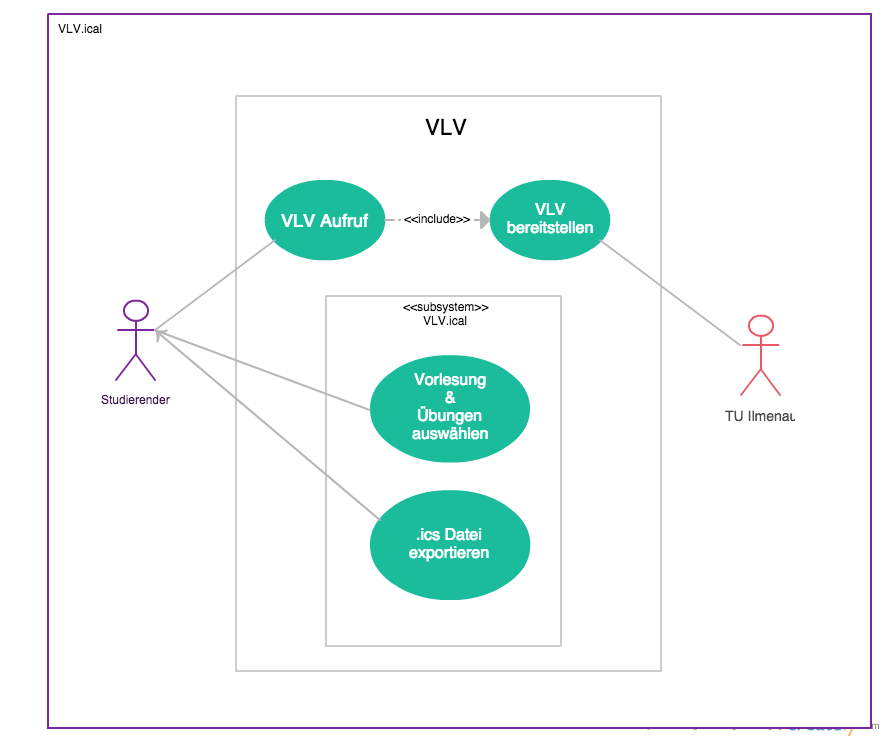
\includegraphics[width=\linewidth]{usecase.png}
    \caption{Use Case Diagramm zu VLV.ical}
\end{figure}
\newpage

\section{Entwurfsziele}
\paragraph{Korrektheit:} Die Aufgaben aller definierten Funktionen sollen wie vorgesehen erfüllt werden.

\paragraph{Zuverlässigkeit:} Ein problemloses Starten und Laufen der Software nach einer Installation soll stets gewährleistet sein.

\paragraph{Verständlichkeit:} Durch eine ausführliche und eindeutige Dokumentation, sowie vollständig kommentierter Quellcode soll die Software leichter zu verstehen sein.

\paragraph{Performanz:} Die Software soll die üblichen Browsing-Gewohnheiten des Nutzers nicht beeinflussen.

\paragraph{Benutzerfreundlichkeit:} Die Bedienung der Software soll größtenteils selbsterklärend sein. Ein Benutzerhandbuch soll überflüssig sein.

\paragraph{Konsistenz} Die Software soll zu jedem Zeitpunkt korrekte Ergebnisse liefern. Im Falle von Problemen und Fehlern soll eine Fehlermeldung, statt falscher Ergebnisse geliefert werden.

\section{Muss-Kriterien}
\begin{itemize}
\item \textbf{M1}: Oberfl\"achenlayout-Erweiterung der Software mittels Browser-Extension in Google Chrome
    \begin{itemize}
    \item Die urspr\"ungliche Oberfläche des Vorlesungsverzeichnisses wird unter anderem um Auswahl- und Downloadfunktionen erweitert, um die Interaktion mit dem Nutzer zu erm\"oglichen.
    \item Durch farbliche Untermalung werden dem benutzer ausgew\"ahlte Elemente visualisiert.
    \item Ein zus\"atzliches Popup Fenster erm\"oglicht die Konfiguration der Erweiterung.
    \end{itemize}
\item \textbf{M2}: Auslesen der Veranstaltungsdaten
    \begin{itemize}
    \item Das Auslesen der Veranstaltungsdaten erfolgt mittels Javascript und Regular Expressions.
    \item Auszulesende Daten sind im einzelnen der Veranstaltungsname, der/die Lesende(r), die Uhrzeit (inklusive Dauer), der Zeitraum (angegeben in Kalenderwochen oder einzelnen Daten) und der Ort.
    \end{itemize}
\item \textbf{M3}: Download einer nach dem vCalender Standard formatierten Datei (Endung: *.ics)
    \begin{itemize}
    \item Es soll dem Benutzer m\"oglich sein, angezeigte Veranstaltungen mit wenigen Klicks in einer fertig konfigurierten *.ics Datei zu speichern, um diese im Anschluss in beliebe Kalenderapplikationen zu importieren.
    \end{itemize}
\item \textbf{M4}: Modifizierung der Website zur besseren Lesbarkeit\textbackslash Bedienung
    \begin{itemize}
    \item Die Verwendung von festen div-Containern oder die fehlende Abgrenzung von einzelnen Elementen innerhalb der Website erschwert dem Betrachter die \"Ubersicht \"uber die Informationen. Um eine \"ubersichtliche Struktur zu gew\"ahrleisten, werden einzelne Elemente voneinander visuell abgetrennt und die wichtigen Informationen hervorgehoben.
    \end{itemize}
\end{itemize}

\section{Wunsch-Kriterien}
\begin{itemize}
\item \textbf{W1}: Erweiterung für andere (Desktop-) Browser portieren
    \begin{itemize}
    \item Nach der Fertigstellung der Erweiterung für Google Chrome könnte eine Portierung auf andere Browser stattfinden.
    \end{itemize}
\item \textbf{W2}: visuelle Hervorhebung der zuletzt aktualisierten Veranstaltungen
    \begin{itemize}
    \item Um dem Benutzer des Vorlesungsverzeichnisses auf \"Anderungen in der Veranstaltungsliste hinzuweisen würde eine visuelle Hervorhebung dieser Veranstaltung ihn darüber informieren, dass in der jeweiligen Veranstaltung k\"urzlich \"Anderungen vorgenommen wurden.
    \end{itemize}
\item \textbf{W3}: Abstraktion des Quellcodes, um eine Anwendung auch außerhalb des VLV zu bieten
    \begin{itemize}
    \item Eine Abstraktion
    \end{itemize}
\end{itemize}

\section{Abgrenzungskriterien}
\begin{itemize}
\item Die Software bietet ausschließlich den Download der angezeigten Informationen als Formatierte *.ics Datei nach dem vCalendar Standard.
\item Die Software liest die Informationen des Vorlesungsverzeichnisses aus und bietet diese nur als formatierte Datei zum Download an.
\item Der Benutzer muss diese formatierte *.ics Datei selbst in den eigenen elektronischen Kalender übernehmen.
\item Grundlage der Informationen ist das Vorlesungsverzeichnis. Sind diese fehlerhaft oder durch menschliches Versagen verfälscht oder inkonsistent, werden diese nicht von der Software abgefangen.
\item Die Software selbst speichert keine Daten, welche Veranstaltungen ausgewählt wurden.
\item Die Software ist ausschließlich für das Vorlesungsverzeichnis der TU-Ilmenau konzipiert. Kompatibilitäten mit anderen Seiten sind durch Softwareentwickler zu portieren.
\item Die Software ist nur mit genannten Browser kompatibel. 
\end{itemize}

\section{Funktionsbeschreibungen}
\paragraph{Download aller Daten für ein Semester}
Die Software soll es ermöglichen, in der Ansicht für ein bestimmtes Semester eines bestimmten Studienganges alle angezeigten Informationen mit einem Klick herunterzuladen.

\paragraph{Download ausgewählter Daten nach dem Warenkorbprinzip}
Die Software soll es aber auch ermöglichen, dass der Benutzer sich nach dem Warenkorbprinzip (siehe Online Shops) Veranstaltungen auswählen kann. Dies soll sowohl Semester-, als auch Studiengangübergreifend möglich sein.

\chapter{Vorgehensmodell - SCRUM}
\section{Allgemeine Definition Scrum}

Scrum kennt drei Rollen für direkt am Prozeß Beteiligte: Product Owner(stellt fachliche Anforderungen und priorisiert sie), ScrumMaster(managt den Prozeß und beseitigt Hindernisse) und Team (entwickelt das Produkt). Daneben gibt es als Beobachter und Ratgeber noch die Stakeholders.

Die Anforderungen (Requirements) werden in einer Liste (Product Backlog) gepflegt, erweitert und priorisiert. Das Product Backlog ist ständig im Fluß. Um ein sinnvolles Arbeiten zu ermöglichen, wird monatlich vom Team in Kooperation mit dem Product Owner ein definiertes Arbeitspaket dem oberen, höher priorisierten Ende des Product Backlogs entnommen und komplett in Funktionalität umgesetzt (inkl. Test und notwendiger Dokumentation). Dieses Arbeitspaket, das Increment, wird während der laufenden Iteration, des sog. Sprints, nicht durch Zusatzanforderungen modifiziert, um seine Fertigstellung nicht zu gefährden. Alle anderen Teile des Product Backlogs können vom Product Owner in Vorbereitung für den nachfolgenden Sprint verändert bzw. neu priorisiert werden.

\begin{figure}[hbt]
    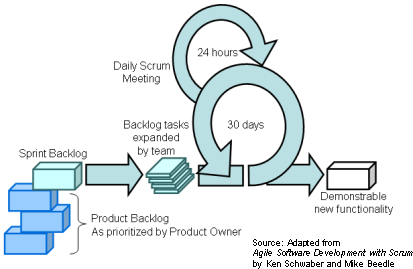
\includegraphics{Scrum.png}
    \caption{Scrum Vorgehensmodell (http://www.torsten-horn.de/img/Scrum.png)}
\end{figure}

Das Arbeitspaket wird in kleinere Arbeitspakete (Tasks) heruntergebrochen und mit jeweils zuständigem Bearbeiter und täglich aktualisiertem Restaufwand in einer weiteren Liste, dem Sprint Backlog, festgehalten.  Während des Sprints arbeitet das Team konzentriert und ohne Störungen von außen daran, die Tasks aus dem Sprint Backlog in ein Increment of Potentially Shippable Functionality, also einen vollständig fertigen und potentiell produktiv einsetzbaren Anwendungsteil, umzusetzen. Das Team gleicht sich in einem täglichen, streng auf 15 Minuten begrenzten Informations-Meeting, dem Daily Scrum Meeting, ab, damit jeder weiß, woran der andere zuletzt gearbeitet hat, was er als nächstes vor hat und welche Probleme es evtl. gibt.

Am Ende des Sprints präsentiert das Team dem Product Owner, den Stakeholders u.a. interessierten Teilnehmern in einem sog. Sprint Review Meeting live am System die implementierte Funktionalität. Halbfertiges oder gar Powerpoint-Folien sind während des Reviews verboten. Das Feedback der Zuseher und die neuen Anforderungen des Product Owners für den kommenden Sprint fließen dann wieder in das nächste Sprint Planning Meeting ein, und der Prozeß beginnt von neuem.

Der ScrumMaster sorgt während des gesamten Prozesses dafür, daß Regeln eingehalten werden und der Status aller Tasks im Sprint Backlog von den jeweils zuständigen Team-Mitgliedern täglich aktualisiert wird. Er macht den Projektfortschritt transparent durch einen geeigneten Reporting-Mechanismus: die Veröffentlichung sog.Burndown Charts, welche den Fortschritt für den aktuellen Sprint bzw. für das gesamte Projekt jeweils in Form einer Kurve visualisieren. Eingezeichnete Trendlinien erlauben es, mögliche Probleme und Verzögerungen einfach (und rechtzeitig!) zu erkennen.

Im Kern basiert Scrum also auf einer inkrementellen Vorgehensweise, der Organisation von Entwicklungsabschnitten und Meetings in vordefinierten Zeitabschnitten (Time-Boxes) und der Erkenntnis, daß ein funktionierendes Produkt wichtiger ist als eine dreihundertseitige Spezifikation.

\newpage
\section{Scrum in Bezug auf das Team}
\paragraph{Entwurfsphase}
\begin{itemize}
\item Project Owner: Cem Kaygusuz
\item ScrumMaster: Norris Sam Osarenkhoe und Erik Langenhan
\item Entwicklerteam: Michael Hähnel, Tim Reinhold, Florian Raetz, Berk Bayraktar, Rajeethan Dhayaparan
\item Stakeholder: Dr. Ing. Talph Maschotta und M. Sc. Thomas Dietrich
\end{itemize}
\paragraph{Implementierung}
\begin{itemize}
\item Project Owner: Erik Langenhan
\item ScrumMaster: Norris Sam Osarenkhoe
\item Entwicklerteam: Michael Hähnel, Tim Reinhold, Florian Raetz, Berk Bayraktar, Rajeethan Dhayaparan, Cem Kaygusuz
\item Stakeholder: Dr. Ing. Talph Maschotta und M. Sc. Thomas Dietrich
\end{itemize}
\paragraph{Validierung}
\begin{itemize}
\item Project Owner: Michael Hähnel
\item ScrumMaster: Berk Bayraktar
\item Entwicklerteam: Tim Reinhold, Florian Raetz, Rajeethan Dayaparan, Norris Sam Osarenkhoe, Erik Langenhan, Cem Kaygusuz
\item Stakeholder: Dr. Ing. Talph Maschotta und M. Sc. Thomas Dietrich
\end{itemize}
\chapter{Verwendete Technologien und Entwicklungswerkzeuge}
\section{Codeverwaltung}
\paragraph{Git \& GitHub}
Der Sourcecode des Projektes wird über Git verwaltet, welches wiederum über das Portal GitHub.com für jeden als freie Software zur Verf\"ugung gestellt wird.
Git ermöglicht es allen, gleichzeitig an der Software zu arbeiten und die \"Anderungen im Anschluss wieder zusammen zu f\"uhren um eine ganzheitliche Software zu erstellen. Sie bietet außerdem eine vollst\"andige History, womit Fehler zu jeder Zeit r\"uckg\"angig gemacht werden k\"onnen.
Des weiteren ist vollst\"andig nachvollziehbar, welche Person zu welchem Zeitpunkt an welchem St\"uck Quellcode gearbeitet hat.

\section{Kommunikation und Organisation}
\paragraph{Gitter.com}
Zur Kommunikation wird haupts\"achlich Gitter genutzt, welches sehr stark mit GitHub.com verkn\"upft ist und somit eine sehr stark projektorientierte Kommunikationsplattform. Sie bietet neben spezieller Textformatierung f\"ur Quellcode auch die Referenzierung auf Personen, Tickets und auch Dateien im Github Projekt. Außerdem sind auf der Plattform aktuelle Aktivit\"aten des Projektes \"uber sogenannte "Git-Hooks" ersichtlich.
\paragraph{WhatsApp}
Zur Organisation von Terminen, Versp\"atungen u.ä. dient außerdem die bekannte Messaging-Applikation WhatsApp.
\paragraph{Trello}
Zur Aufgabenverteilung, -zuweisung und auch zur Fortschrittsanalyse wird das Online-Portal Trello.com genutzt. Durch eine Browser Erweiterung bietet es außerdem eine Unterstützung des Vorgehensmodells SCRUM.

\section{Programmiersprachen}
\paragraph{Javascript}
Da es sich bei diesem Projekt um eine Browser Erweiterung handelt, wird hauptsächlich die Programmiersprache Javascript zum Einsatz kommen.
\paragraph{HTML}
HTML dient zur Darstellung aller Inhalte, die durch die Erweiterung neu hinzugefügt werden.
\paragraph{Bibliotheken}
Um die grundlegenden Möglichkeiten von Javascript zu erweitern werden wir uns an freien Javascript Bibliotheken, wie z.B. jQuery und möglicherweise noch anderen bedienen.

\chapter{Glossar}
\paragraph{Git} Git ist eine freie Software zur verteilten Versionsverwaltung von Dateien, die ursprünglich von Linux-Entwickler Linus Torvalds entwickeld wurde, um den Source Code des Linux Kernels zu verwalten.

\paragraph{GitHub.com} GitHub ist ein Portal, um Git Projekte zu hosten. Es bietet eine übersichtliche Oberfläche und erweitert das pure Git um weitere Projektmanagementfunktionen, wie eine Ticket (engl. Issue) Funktion und Analyse Funktionen.

\paragraph{Product Owner}
Die für die Pflege des Product Backlogs verantwortliche Person

\paragraph{ScrumMaster}
Die für den Scrum-Prozeß verantwortliche Person

\paragraph{Stakeholders}
Jemand, der ein besonderes Interesse am Projektergebnis hat.

\paragraph{Requirements}
Funktionale oder nicht-funktionale Anforderung an das Produkt .

\paragraph{Product Backlog}
Priorisierte Liste von Anforderungen

\paragraph{Increment} 
Produktfunktionalität die während eines Sprint entwickelt wird .

\paragraph{Sprints}
Eine Time-Box von 30 aufeinanderfolgenden Kalendertagen.

\paragraph{Sprint Backlog}
Eine Liste von Aufgaben, die den Umfang des Sprint festlegt.

\paragraph{Daily Scrum}
Kurzes, tägliches Status-Meeting

\paragraph{Sprint Review Meeting} 
Meeting am Ende eines  Sprints.

\paragraph{Burndown Charts}
Graphik, die den Projektfortschritt zeigt.

\paragraph{Time-Boxes}Ein streng einzuhaltendes Zeitfenster

\end{document}
